\chapter{ideal Bose systems} \label{7}
\begin{itemize}
	\item 根据 \eqref{5.4.2}, 如果 $n \lambda^3 \ll 1$ 的条件不再满足, 就需要考虑量子效应.
	\begin{itemize}
		\item 需要分别讨论可以对 $n \lambda^3 \lesssim 1$ 作级数展开的区间, 和 $n \lambda^3 \gtrsim 1$ 系统完全偏离经典统计的情况.
	\end{itemize}
	
	\item $g_n(z)$ 是 Bose--Einstein function,
	\begin{equation}
		g_n(z) \equiv \frac{1}{\Gamma(n)} \int_0^\infty \frac{x^{n - 1}}{z^{- 1} e^x - 1} dx = z + \frac{z^2}{2^n} + \frac{z^3}{3^n} + \cdots, \quad \text{and} \quad g_n'(z) = \frac{1}{z} g_{n - 1}(z),
	\end{equation}
	是单调递增函数, $- 1 < z < 1$, 且 $g_n(1) = \zeta(n)$.
\end{itemize}

\section{thermodynamic behavior of an ideal Bose gas} \label{7.1}
\begin{itemize}
	\item ideal Bose gas 的 grand partition function 为
	\begin{equation} \label{7.1.1}
		\frac{P V}{k_B T} = \ln Z_\text{GC} = N_s \Big( \frac{V}{\lambda^3} g_{5 / 2}(z) - \underbrace{\ln(1 - z)}_{\text{negligible}} \Big),
	\end{equation}
	其中 $z = e^{\beta \mu} < 1$ 是 fugacity (见 \eqref{1.3.3}), $N_s$ 是粒子的自旋状态数.
	
	\begin{tcolorbox}[title=calculation:]
		注意到粒子能量 $\epsilon$ 的简并度为 (根据 \eqref{1.2.3})
		\begin{equation} \label{7.1.2}
			g(\epsilon) = N_s 2 \pi \frac{V / \lambda^3}{(\pi k_B T)^{3 / 2}} \epsilon^{1 / 2},
		\end{equation}
		所以 (另外 $g_0 = N_s \neq 0$, 而 $g(0) = 0$, 需要把 $\epsilon = 0$ 单独拿出来)
		\begin{align}
			\ln Z_\text{GC} &= - N_s \ln(1 - z) - N_s 2 \pi \frac{V / \lambda^3}{(\pi k_B T)^{3 / 2}} \int_0^\infty \ln(1 - z e^{- \beta \epsilon}) \epsilon^{1 / 2} d\epsilon \notag \\
			&= - N_s \ln(1 - z) - N_s \frac{2 \pi}{\pi^{3 / 2}} \frac{V}{\lambda^3} \int_0^\infty \ln(1 - z e^{- x}) x^{1 / 2} dx = \cdots,
		\end{align}
		注意 $\ln(1 - z)$ 在 $z = 1$ 处有一个极点, 所以 Taylor 展开收敛的条件是
		\begin{equation} \label{7.1.4}
			z e^{- x} < 1 \Longrightarrow z < 1.
		\end{equation}
	\end{tcolorbox}
	
	\begin{itemize}
		\item 基态贡献的 $N_s \ln(1 - z)$ 可以忽略 (但其导数不一定能忽略).
		
		\begin{tcolorbox}[title=proof:]
			注意到
			\begin{equation}
				N_0 = N_s \frac{1}{z^{- 1} - 1} \Longrightarrow - N_s \ln(1 - z) = N_s \ln(N_0 / N_s + 1) \leq O(\ln N),
			\end{equation}
			而 $\ln Z_\text{GC} \sim N$, 因此可以忽略.
		\end{tcolorbox}
	\end{itemize}
	
	\item 得到 (框起来的公式在 $T_c$ 两侧都成立)
	\begin{equation}
		\boxed{\begin{dcases}
			N = N_s \frac{V}{\lambda^3} g_{3 / 2}(z) + N_s \frac{1}{z^{- 1} - 1} \\
			U = \frac{3 N_s}{2} k_B T \frac{V}{\lambda^3} g_{5 / 2}(z)
		\end{dcases}},
	\end{equation}
	和 equation of state (in the form of virial expansion, 见 \eqref{3.5.12}),
	\begin{equation}
		\boxed{\frac{P V}{N k_B T} = \frac{1}{n \lambda^3 / N_s} g_{5 / 2}(z)} = \begin{dcases}
			\frac{g_{5 / 2}(z)}{g_{3 / 2}(z)} = \sum_{l = 1}^\infty a_l (n \lambda^3 / N_s)^{l - 1} & T \gg T_c, \ \text{virial expansion} \\
			\frac{1}{n \lambda^3 / N_s} \zeta({\textstyle \frac{5}{2}}) & T < T_c
		\end{dcases},
	\end{equation}
	($T \gg T_c$ 指要求级数收敛), 其中 virial coefficients are
	\begin{align}
		& a_1 = 1, \quad a_2 = - \frac{1}{4 \sqrt{2}} \approx - 0.177, \quad a_3 = - \Big( \frac{2}{9 \sqrt{3}} - \frac{1}{8} \Big) \approx - 0.0033, \notag \\
		& a_4 = - \Big( \frac{3}{32} + \frac{5}{32 \sqrt{2}} - \frac{1}{2 \sqrt{6}} \Big) \approx - 0.00011. \label{7.1.8}
	\end{align}
	
	\item 注意到 $U = \frac{3}{2} P V$ ($T < T_c$ 时也成立), 系统的 specific heat 为
	\begin{equation}
		\frac{C_V}{N k_B} = \begin{dcases}
			\overbrace{\frac{15}{4} \frac{g_{5 / 2}(z)}{g_{3 / 2}(z)} - \frac{9}{4} \frac{g_{3 / 2}(z)}{g_{1 / 2}(z)}}^{\text{忽略了} \ N_0} = \frac{3}{2} \sum_{l = 1}^\infty \frac{5 - 3 l}{2} a_l (n \lambda^3 / N_s)^{l - 1} & T \gg T_c \\
			\frac{15}{4} \frac{\zeta({\textstyle \frac{5}{2}})}{\zeta({\textstyle \frac{3}{2}})} \Big( \frac{T}{T_c} \Big)^{\frac{3}{2}} & T < T_c
		\end{dcases}.
	\end{equation}
	
	\item 得到 $T$--$P V$ 和 $T$--$C_V$ 曲线, 如下图:
	
	\begin{figure}[H]
		\centering
		\begin{subfigure}{0.4\linewidth}
			\centering
			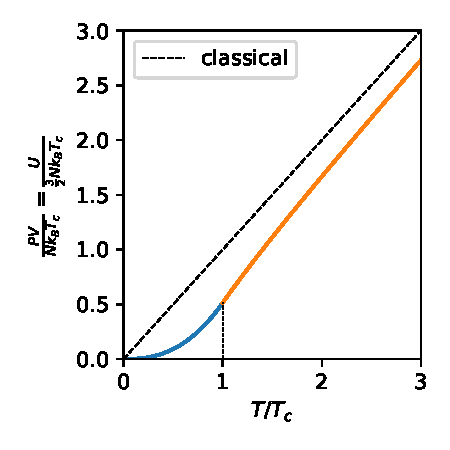
\includegraphics[scale=0.8]{figures/plot of T--PV.pdf}
			\caption{plot of $T$--$P V$.}
		\end{subfigure}
		\begin{subfigure}{0.4\linewidth}
			\centering
			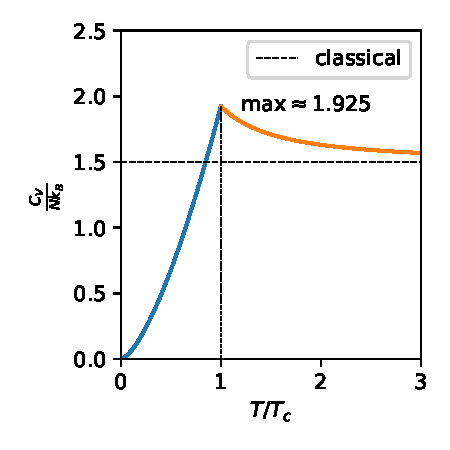
\includegraphics[scale=0.8]{figures/plot of T--C_V.pdf}
			\caption{plot of $T$--$C_V$.}
		\end{subfigure}
		\caption{}
	\end{figure}
	
	可见 $T = T_c$ 时存在相变.
	
	\item 系统的熵为
	\begin{equation} \label{7.1.10}
		S = U + P V - \mu N = \begin{dcases}
			N k_B \Big( \frac{5}{2} \frac{g_{5 / 2}(z)}{g_{3 / 2}(z)} - \ln z \Big) & T > T_c \\
			\frac{5}{2} k_B \frac{V}{\lambda^3 / N_s} \zeta({\textstyle \frac{5}{2}}) = \frac{5}{2} k_B N_e \frac{\zeta(\frac{5}{2})}{\zeta(\frac{3}{2})} & T < T_c
		\end{dcases},
	\end{equation}
	可见 $S \propto N_e$, 处于基态的粒子不贡献熵, as expected.
\end{itemize}

\subsection{normal phase and condensed phase}
\begin{itemize}
	\item grand partition function 计算方法的前提条件是 \eqref{7.1.4}, (代入 $N$-$z$ 关系式) 等价于
	\begin{equation}
		N_e < N_s \frac{V}{\lambda^3} \underbrace{\zeta({\textstyle \frac{3}{2}})}_{\approx 2.612},
	\end{equation} 
	其中 $N_e$ 表示激发态上的粒子数量.
	
	\item 当 $z$ 接近 $1$ 时, $N_0 = N_s \frac{1}{z^{- 1} - 1} \gg 1$, 此时,
	\begin{equation}
		\begin{dcases}
			z = 1 - \frac{N_s}{N_0} \\
			N_0 = N - N_s \frac{V}{\lambda^3} \zeta({\textstyle \frac{3}{2}}) \gg 1
		\end{dcases},
	\end{equation}
	几乎所有粒子都处于基态, 称为 Bose--Einstein condensation.
	
	\item 发生 Bose--Einstein condensation 的条件是 $N > N_s \frac{V}{\lambda^3} \zeta(\frac{3}{2})$, 或者
	\begin{equation}
		n \lambda^3 / N_s > \zeta({\textstyle \frac{3}{2}}) \iff T < T_c = \frac{h^2}{2 \pi m k_B} \Big( \frac{N / N_s}{V \zeta(\frac{3}{2})} \Big)^{\frac{2}{3}},
	\end{equation}
	此时, 系统可以认为处于两相混合态: 由 $N_e$ 个处于激发态的粒子 (in the normal phase), 和 $N_0$ 个处于基态的粒子 (in the condensed phase) 组成.
	\begin{itemize}
		\item 一个对化简有用的公式,
		\begin{equation}
			\frac{T}{T_c} = \Big( \frac{\zeta(\frac{3}{2})}{n \lambda^3 / N_s} \Big)^{\frac{2}{3}}.
		\end{equation}
		
		\item $T < T_c$ 时,
		\begin{equation}
			\frac{N_0}{N} = 1 - \Big( \frac{T}{T_c} \Big)^{\frac{3}{2}} \overset{T = T_c - 0^+}{\approx} \frac{3}{2} \frac{T_c - T}{T_c}.
		\end{equation}
	\end{itemize}
	
	\item 综上, $z$ 随 $T$ 变化曲线如 figure \ref{figure 7.2 (a)}.
	
	\begin{figure}[H]
		\centering
		\begin{subfigure}{0.4\linewidth}
			\centering
			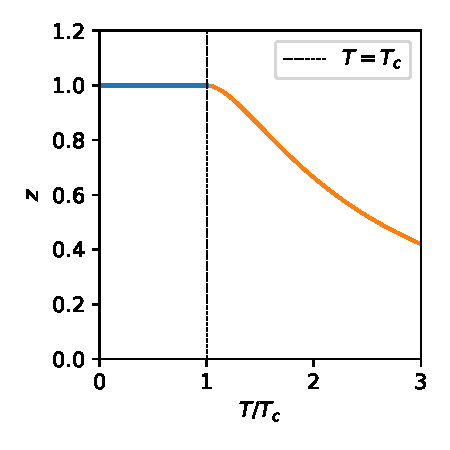
\includegraphics[scale=0.8]{figures/plot of T--z.pdf}
			\caption{plot of $T$--$z$.}
			\label{figure 7.2 (a)}
		\end{subfigure}
		\begin{subfigure}{0.4\linewidth}
			\centering
			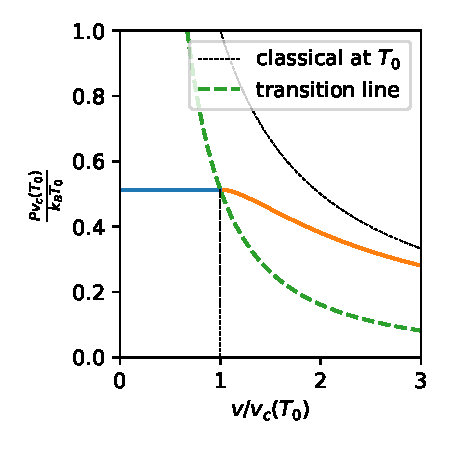
\includegraphics[scale=0.8]{figures/plot of an isotherm at T_0.pdf}
			\caption{plot of an isotherm at $T_0$.}
			\label{figure 7.2 (b)}
		\end{subfigure}
		\caption{}
	\end{figure}
\end{itemize}

\subsection{isotherms and adiabats of the ideal Bose gas}
\begin{itemize}
	\item 等温线上, 相变发生在 characteristic volume,
	\begin{equation}
		v_c = \frac{\lambda^3}{N_s \zeta(\frac{3}{2})},
	\end{equation}
	因此, $v$--$P$ 曲线如 figure \ref{figure 7.2 (b)}, 其中 transition line 为
	\begin{equation}
		P v^{5 / 3} = \frac{h^2}{2 \pi m} \frac{1}{N_s^{2 / 3}} \frac{\zeta(\frac{5}{2})}{\zeta^{5 / 3}(\frac{3}{2})},
	\end{equation}
	是一条特殊的绝热线.
	
	\item 可逆绝热过程中, 根据 \eqref{7.1.10},
	\begin{align}
		& \begin{dcases}
			z = \text{Const.} \Longrightarrow n \lambda^3 = \text{Const.} & T > T_c \\
			n \lambda^3 = \text{Const.} & T < T_c
		\end{dcases} \notag \\
		\Longrightarrow & n \lambda^3 = \text{Const.} \quad \text{or} \quad \frac{P}{T^{5 / 2}} = \text{Const.} \quad \text{or} \quad P v^{5 / 3} = \text{Const.},
	\end{align}
	与 ideal classical gas 中的情况完全一样, 但是
	\begin{equation}
		\gamma \equiv \frac{C_P}{C_V} = \frac{5}{3} \frac{g_{5 / 2}(z) g_{1 / 2}(z)}{g_{3 / 2}^2(z)},
	\end{equation}
	与 ideal classical gas 中不一样.
\end{itemize}

\section{Bose--Einstein condensation in ultracold atomic gases} \label{7.2}
\begin{itemize}
	\item 考虑单个粒子的 Hamiltonian 为
	\begin{equation}
		H = \frac{|\vec{p}|^2}{2 m} + V(\vec{r}), \quad V(\vec{r}) = \frac{1}{2} m (\omega_x^2 x^2 + \omega_y^2 y^2 + \omega_z^2 z^2),
	\end{equation}
	粒子的能级为
	\begin{equation}
		\epsilon = \sum_i \hbar \omega_i \Big( n_i + \frac{1}{2} \Big).
	\end{equation}
	
	\item 系统的 grand partition function 为
	\begin{equation}
		\ln Z_\text{GC} = - N_s \Big( \frac{1}{2 (\beta \hbar \omega_0)^3} g_4(z) + \underbrace{\ln(1 - z e^{- \beta \epsilon_0})}_{\text{negligible}} \Big).
	\end{equation}
	
	\begin{tcolorbox}[title=calculation:]
		注意到
		\begin{equation}
			\int_0^\epsilon g(\epsilon') d\epsilon' = N_s \int \theta(\epsilon - \epsilon(\vec{n})) d^3 n,
		\end{equation}
		因此, 能级 $\epsilon \gg \epsilon_0$ 的简并为
		\begin{align}
			g(\epsilon) &= N_s \int_0^\infty dn_1 \int_0^\infty dn_2 \int_0^\infty dn_3 \, \delta(\epsilon - \epsilon(n_1, n_2, n_3)) \notag \\
			&= N_s \int_0^\infty dn_1 \int_0^\infty dn_2 \, \frac{1}{\hbar \omega_3} \theta(\epsilon - \epsilon(n_1, n_2, 0)) \notag \\
			&= N_s \frac{1}{\hbar \omega_3} \int_0^{\frac{(\epsilon - \epsilon_0)}{\hbar \omega_1}} dn_1 \int_0^{\frac{(\epsilon - \epsilon_0) - \hbar \omega_1 n_1}{\hbar \omega_2}} dn_2 \, 1 = N_s \frac{(\epsilon - \epsilon_0)^2}{2 (\hbar \omega_0)^3},
		\end{align}
		其中 $\omega_0 = (\omega_1 \omega_2 \omega_3)^{1 / 3}$, 且基态能量 $\epsilon_0$ 可以忽略. 代入 \eqref{6.1.10},
		\begin{align}
			\ln Z_\text{GC} &= - N_s \ln(1 - z e^{- \beta \epsilon_0}) - \int_0^\infty \ln(1 - z e^{- \beta \epsilon}) g(\epsilon) d\epsilon \notag \\
			&= - N_s \ln(1 - z e^{- \beta \epsilon_0}) - N_s \frac{1}{2 (\beta \hbar \omega_0)^3} \int_0^\infty \ln(1 - z e^{- x}) x^2 dx = \cdots
		\end{align}
	\end{tcolorbox}
	
	\item 得到
	\begin{equation}
		\begin{dcases}
			N = N_s \frac{1}{(\beta \hbar \omega_0)^3} g_3(z) + N_s \frac{1}{z^{- 1} - 1} \Longrightarrow \frac{k_B T_c}{\hbar \omega_0} = \Big( \frac{N / N_s}{\zeta(3)} \Big)^{\frac{1}{3}} \\
			U = 3 \frac{(k_B T)^4}{(\hbar \omega_0)^3} g_4(z) \\
			\frac{C_\omega}{N k_B} = \begin{dcases}
				\frac{12 \zeta(4)}{\zeta(3)} \Big( \frac{T}{T_c} \Big)^3 \\
				\frac{1}{\zeta(3)} \Big( \frac{T}{T_c} \Big)^3 \Big( 12 g_4(z) - \frac{9 g_3^2(z)}{g_2(z)} \Big)
			\end{dcases}
		\end{dcases},
	\end{equation}
	其中 $C_\omega$ 不连续, 与 section \ref{7.1} 中不同.
\end{itemize}

\section{thermodynamics of the blackbody radiation: the photon gas} \label{7.3}
\begin{itemize}
	\item section \ref{4.1} 中的推导前提是 heat reservoir 粒子数守恒, photon gas 没有这个约束条件, 因此 $\mu = 0$.
	
	\item photon 的能级为
	\begin{equation}
		\epsilon = \frac{h c}{2 L} \sqrt{n_x^2 + n_y^2 + n_z^2}.
	\end{equation}
	
	\item photon gas 的 grand partition function 为
	\begin{equation}
		\frac{P V}{k_B T} = \ln Z_\text{GC} = 16 \pi \frac{V}{h^3 c^3} (k_B T)^3 g_4(z) \Big|_{z = 1} = \frac{8 \pi^5 V}{45 h^3 c^3} (k_B T)^3,
	\end{equation}
	虽然 $z = 1$, 但 $\ln Z_\text{GC}(T, V, z)$ 对 $z$ 的偏导数依然有用.
	
	\begin{tcolorbox}[title=calculation:]
		能级简并为
		\begin{align}
			g(\epsilon) &= 2 \int_0^\infty dn_1 \int_0^\infty dn_2 \int_0^\infty dn_3 \, \delta(\epsilon - \epsilon(n_1, n_2, n_3)) \notag \\
			&= 2 \int_0^\infty dn_1 \int_0^\infty dn_2 \, \Big( \frac{h c}{2 L} \frac{n_3}{\sqrt{n_1^2 + n_2^2 + n_3^2}} \Big|_{\epsilon = \epsilon(\vec{n})} \Big)^{- 1} \theta(\epsilon - \epsilon(n_1, n_2, 0)) \notag \\
			&= 2 \epsilon \Big( \frac{2 L}{h c} \Big)^2 \int_0^\infty dn_1 \int_0^\infty dn_2 \, \frac{1}{\sqrt{n_\epsilon^2 - n_1^2 - n_2^2}} \theta(\epsilon - \epsilon(n_1, n_2, 0)) = 8 \pi \frac{V}{h^3 c^3} \epsilon^2,
		\end{align}
		代入 \eqref{6.1.10},
		\begin{align}
			\ln Z_\text{GC} &= - 2 \ln(1 - z) - \int_0^\infty \ln(1 - z e^{- \beta \epsilon}) g(\epsilon) d\epsilon \notag \\
			&= - 2 \ln(1 - z) + 16 \pi \frac{V}{h^3 c^3} (k_B T)^3 g_4(z),
		\end{align}
		忽略第一项, 令 $z = 1, \zeta(4) = \frac{\pi^4}{90}$, 得到...
	\end{tcolorbox}
	
	\item 得到
	\begin{equation}
		\begin{dcases}
			N = \frac{\partial}{\partial \alpha} \Big|_{\alpha = 0} \ln Z_\text{GC} = \int_0^\infty \frac{g(\epsilon)}{e^{\beta \epsilon} - 1} d\epsilon = 16 \pi \zeta(3) \frac{V}{h^3 c^3} (k_B T)^3 \\
			\frac{U}{V} = 3 P = \frac{8 \pi^5}{15} \frac{1}{h^3 c^3} (k_B T)^4 \\
			S = \frac{4}{3} \frac{U}{T} \\
			C_V = 3 S, C_P \rightarrow \infty
		\end{dcases},
	\end{equation}
	以及
	\begin{equation}
		\frac{\braket{(\Delta N)^2}}{\braket{N}^2} = \frac{1}{\braket{N}^2} \frac{\partial^2}{\partial \alpha^2} \Big|_{\alpha = 0} \ln Z_\text{GC} = \frac{1}{\braket{N}} \frac{\pi^2}{6 \zeta(3)},
	\end{equation}
	与 \eqref{4.4.2} 不同 (注意到 photon gas 的 $\kappa_T \rightarrow \infty$).
\end{itemize}

\section{the field of sound waves: the phonon gas} \label{7.4}
\begin{itemize}
	\item 固体的 Hamiltonian 为
	\begin{equation}
		H = \frac{m}{2} \sum_{i = 1}^{3 N} \dot{x}_i^2 + \Phi_0 + \frac{1}{2} \sum_{i, j} \underbrace{\frac{\partial^2 \Phi}{\partial x_i \partial x_j}}_{= \alpha_{i j}} x_i x_j + O(x^3),
	\end{equation}
	其中 $x$ 是固体中的原子相对平衡位置的偏离, 保留二阶项称作 harmonic approximation. 对 $x$ 作正交变换得到 normal coordinates $q$, 得到
	\begin{equation}
		H = \Phi_0 + \sum_{i = 1}^{3 N} \frac{1}{2} m (\dot{q}_i^2 + \omega_i^2 q_i^2),
	\end{equation}
	where $\omega_i$ are the characteristic frequencies of the normal modes.
	
	\item 固体的能级为
	\begin{equation}
		E\{n_i\} = \Phi_0 + \sum_{i = 1}^{3 N} \hbar \omega_i \Big( n_i + \frac{1}{2} \Big).
	\end{equation}
	
	\item 可以认为 $\hbar \omega_i$ 是 phonon 的能级, $n_i$ 是这个能级上的声子数, 那么声子是 indistinguishable Boson, 且粒子数不守恒, $\mu = 0$.
	
	\item 系统的 grand partition function 为
	\begin{equation}
		\ln Z_\text{GC} = - \sum_{i = 1}^{3 N} \ln(1 - z e^{- \beta \hbar \omega_i}) \Big|_{z = 1}.
	\end{equation}
	
	\item 得到
	\begin{equation}
		\begin{dcases}
			N_\text{phonons} = \sum_{i = 1}^{3 N} \frac{1}{e^{\beta \hbar \omega_i} - 1} \\
			U = \Big( \Phi_0 + \sum_{i = 1}^{3 N} \frac{1}{2} \hbar \omega_i \Big) + \sum_{i = 1}^{3 N} \frac{\hbar \omega_i}{e^{\beta \hbar \omega_i} - 1} \\
			C_V = k_B \sum_{i = 1}^{3 N} \frac{e^{\beta \hbar \omega_i}}{(e^{\beta \hbar \omega_i} - 1)^2} (\beta \hbar \omega_i)^2
		\end{dcases}.
	\end{equation}
	
	\item 进一步的研究依靠固体的 frequency spectrum, Einstein 假设 $\omega_1 = \cdots = \omega_{3 N} = \omega_E$, Debye 假设固体有 continuous spectrum of frequencies.
\end{itemize}

\subsection{Einstein solid model}
\begin{itemize}
	\item 代入 $\omega_i = \omega_E$, 令 $\hbar \omega_E = k_B \Theta_E$, 得到
	\begin{equation}
		C_V = 3 N k_B \frac{e^{\Theta_E / T}}{(e^{\Theta_E / T} - 1)^2} (\Theta_E / T)^2.
	\end{equation}
\end{itemize}

\subsection{Debye solid model}
\begin{itemize}
	\item Debye 假设 phonon 的能级简并为
	\begin{equation}
		g(\omega) \equiv g(\epsilon) \frac{d\epsilon}{d\omega} = \begin{dcases}
			9 N \frac{\omega^2}{\omega_D^3} & \omega \leq \omega_D \\
			0 & \omega > \omega_D
		\end{dcases}, \quad \omega_D^3 = 18 \pi^2 \frac{N}{V} \Big( \frac{1}{c_L^3} + \frac{2}{c_T^3} \Big)^{- 1},
	\end{equation}
	其中 $c_L, c_T$ 分别是固体中 longitude modes 和 transverse modes 的声速.
	
	\begin{tcolorbox}[title=calculation:]
		声子在固体中形成驻波,
		\begin{equation}
			\frac{\omega_i L}{c} = \pi \sqrt{n_{i, x}^2 + n_{i, y}^2 + n_{i, z}^2} \Longrightarrow g(\omega) = \frac{N_s}{2 \pi^2} \frac{V}{c^3} \omega^2,
		\end{equation}
		注意到横波有两个偏振,
		\begin{equation}
			g(\omega) = \frac{V}{2 \pi^2} \Big( \frac{1}{c_L^3} + \frac{2}{c_T^3} \Big) \omega^2,
		\end{equation}
		总状态为 $3 N$, 所以需要有一个截至频率 $\omega_D$,
		\begin{equation}
			\int_0^{\omega_D} g(\omega) d\omega = 3 N \Longrightarrow \frac{V}{2 \pi^2} \Big( \frac{1}{c_L^3} + \frac{2}{c_T^3} \Big) \frac{\omega_D^3}{3} = 3 N.
		\end{equation}
	\end{tcolorbox}
	
	\item 代入, 令 $\hbar \omega_D = k_B \Theta_D$, 得到
	\begin{equation}
		C_V = 9 N k_B \Big( \frac{T}{\Theta_D} \Big)^3 \int_0^{\Theta_D / T} \frac{x^4 e^x}{(e^x - 1)^2} dx \overset{T \ll \Theta_D}{\approx} \frac{12 \pi^4}{5} N k_B \Big( \frac{T}{\Theta_D} \Big)^3.
	\end{equation}
	
	\item 实验表明固体 (aluminum) 的频谱在低频接近 Debye 的假设, Cu 的 $T$-$C_V$ 曲线在整个实验区间都与 Debye 的预测符合良好.
	
	\item 令 $\omega_E \approx \omega_D$, 固体的比热如下图:
	
	\begin{figure}[H]
		\centering
		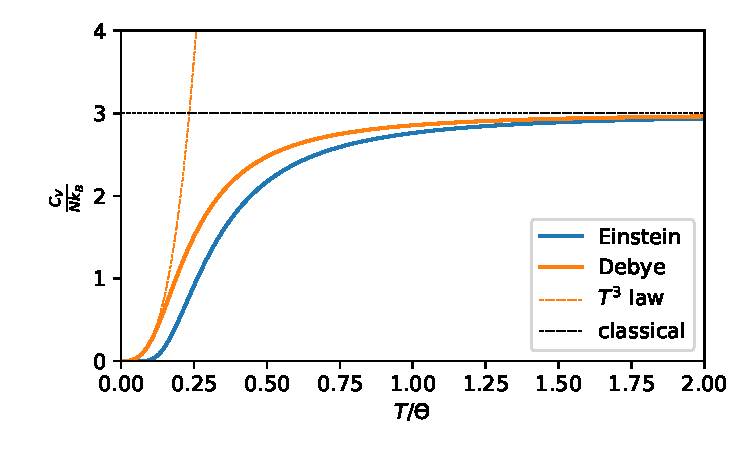
\includegraphics[scale=0.8]{figures/the specific heat of a solid.pdf}
		\caption{the specific heat of a solid.}
		\label{figure 7.3}
	\end{figure}
\end{itemize}

\section{something about helium-4}
\begin{itemize}
	\item about \isotope[4]{He}...
\end{itemize}
